\section{Beyond Standard Model Physics}

Despite it's massive success in predicting the fundamental particles and their interactions in collider experiments, the SM has found its limitations as it fails to provide an explanation to several observed phenomena in particle physics such as the hierarchy problem of the Higgs mass, neutrino oscillations, asymmetry between matter and antimatter and the origin of dark matter. 

Consecutive astrophysics observations dating back to the 1930s have shown time and time again evidence of the existence of non-visible matter or dark matter in the universe. The gravitational pull of dark matter provides an explanation to observations of velocity dispersion of galaxies in clusters not possible by visible matter, to observations of gravitational lensing, to fluctuations in the cosmic microwave background (CMB), and other astrophysics observations. However this evidence does little to pinpoint what dark matter is. SM elementary particles fail to explain the observations as these particles would be sufficiently visible trough electromagnetic interactions or lack the mass (neutrinos) to be considered as dark matter candidates. Extensions of the SM are thus required to introduce new particles that could explain the nature of dark matter. Various SM extensions are considered in indirect dark matter searches in astrophysics observations as well as direct searches with high energy collision experiments at LHC.\\
\\
The hierarchy problem of the Higgs mass is another question raised by the SM, namely why is the Higgs mass so much less than expected. The Higgs mass has no symmetry within the SM that protects it from unstable quantum corrections(Fig. \ref{Fig:Higgs Corrections}), unlike the gauge bosons which are limited to an EWSB energy scale $\mathcal{O}(100\text{GeV})$. One would thus expect the Higgs mass to be of an order $\Lambda$ where new physics (NP) appears. In continuation of the succes of electroweak unification, the “grand unified theory” (GUT) is such NP which unifies the strong and the electroweak interactions. Extrapolation of the strong and electroweak interaction strengths gives a GUT energy scale $\Lambda_{\text{GUT}}$ of $ 10^{16}$GeV, an order $10^{14}$GeV larger than the observed Higgs mass. It is possible within the framework of the SM to explain this low Higgs mass trough a precise fine tuning of the bare Higgs mass $m_0$. We may say in this case that the Higgs mass is an input of the SM to fine tune the bare Higgs mass and it is conceivable that the universe operates in this way. However, we know from other sources that physics beyond the SM must exist and a more elegant solution to the hierarchy problem can find itself in these beyond SM theories.  
\begin{figure}[t]
    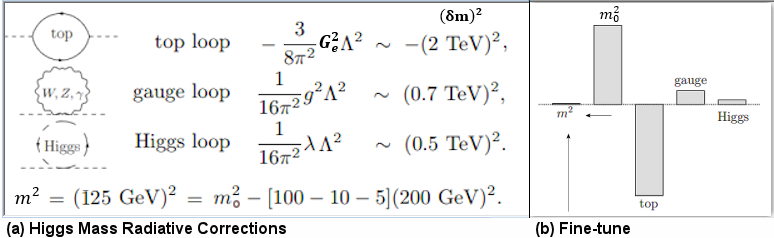
\includegraphics[width=1.0\textwidth]{Figures/HiggsMass.png}
    \caption{Caption}
    \label{Fig:Higgs Corrections}
\end{figure}
The open questions on the SM have led to the development of new physics theories that go beyond the Standard Model. A notable example is supersymmetry which is a new symmetry on top of the SM between fermions and bosons. A strong motivation of SUSY finds itself in new SUSY particles as dark matter candidates and solving the fine-tuning problem discussed above, provided that the new SUSY particles are of EWSB scale. In general a large portion of particles from new physics theories are predicted within the reach of the LHC collision energy. Nonetheless there has yet to be experimental evidence of new physics with direct searches at the LHC, highlighting the importance of alternative indirect searches for new physics at higher energy scales. 

Effective field theory (EFT) is a framework for undertaking indirect searches for BSM physics. This framework constructs a low-energy effective theory of a BSM theory that describes the interactions between particles at energies within the reach of the LHC. The theoretical approach to construct an EFT can be classified in two theories of EFT models: the "bottom-up EFT" and "top-down EFT". In the "top-down EFT", the low-energy EFT is constructed by starting from a well-defined higher-energy theory, such as GUTs. The  high-energy degrees of freedom are integrated out to retain only those degrees of freedom that are relevant for predictions of observables at collider experiment energies. The "bottom-up EFT" model or standard model effective field theory (SMEFT) starts from the SM theory Lagrangian adding higher-dimensional operators that approximate the effect of higher-energy theories in the low-energy EFT Lagrangian:
\begin{equation}\label{EFT Lagrangian}
    \mathscr{L}_{EFT} = \mathscr{L}_{SM} + \sum_{d,i}\frac{c^d_i}{\Lambda^{d-4}}\mathcal{O}^d_i
\end{equation}
where the dimension-d EFT contributions $\mathcal{O}^d_i$ are SM fields that preserve the symmetries of the SM and are suppressed by the higher-energy theory energy scale $\Lambda^{d-4}$. A prime contribution from BSM physics are provided by dimension-six EFT operators. By measuring observables that are sensitive to the effects of the EFT such as deviations from SM cross section predictions we can probe BSM physics, i.e. constraining coefficients of higher-dimensional operators in the EFT. SMEFT does not require detailed knowledge of a specific high-energy theory and thus is model independent, making it the preferred method in BSM physics searches at LHC. In the context of rare top quark processes, the masters thesis topic, observables of processes involving the production of top quarks in association with a W, Z, or Higgs boson are exceptionally sensitive to EFT operators. This is due to the large mass of the top quark, and therefore its large coupling to the Higgs boson, being a possible indication of a special relationship between the top quark and the physics of EWSB not yet understood by the SM. Recent experimental measurements on EFT operators in rare top quark processes as well as the connection to the masters thesis topic are discussed in the state-of-the-art chapter.